\usetikzlibrary{positioning,arrows}
\usetikzlibrary{decorations.pathmorphing}
\usetikzlibrary{decorations.markings}
\usetikzlibrary{math,calc}

\tikzset{
    midarrow/.style={draw, postaction={decorate},
        decoration={markings,mark=at position .55 with {\arrow[draw]{>}}}},
    midarrow-rev/.style={draw, postaction={decorate},
        decoration={markings,mark=at position .55 with {\arrow[draw]{<}}}},
}

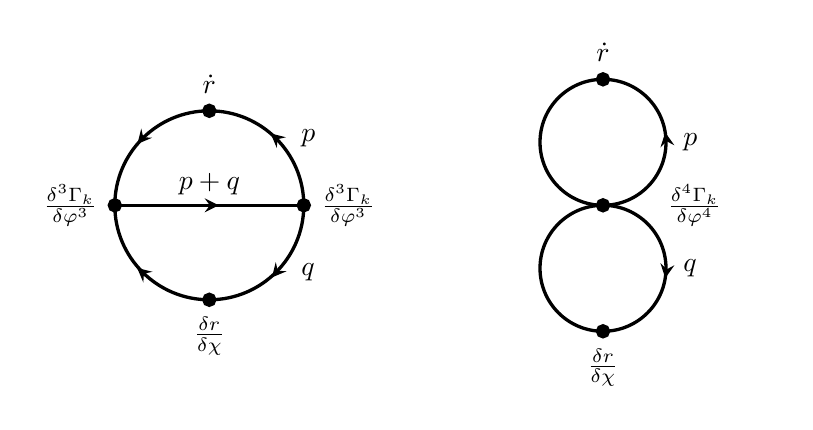
\begin{tikzpicture}[
    >=stealth,
    scale=1.00,
    very thick,
  ]

  \tikzmath{
    \lradius   = 1.2; % radius of left circle
    \rradius   = 0.8; % radius of right circle
    \dotradius = 0.07; % radius of the circles that make the dots
  }

  \coordinate (dist) at (5,0); % define the distance between the two Feynman diagrams

  % -------------
  % First Diagram
  % -------------

  % The circle with four segments
  \draw[midarrow]     (\lradius, 0) arc (  0:  90: \lradius) node[midway, right, inner sep=0.3cm] {$p$};
  \draw[midarrow]     (0, \lradius) arc ( 90: 180: \lradius);
  \draw[midarrow-rev] (-\lradius,0) arc (180: 270: \lradius);
  \draw[midarrow-rev] (0,-\lradius) arc (270: 360: \lradius) node[midway, right, inner sep=0.3cm] {$q$};

  % Line in the middle
  \draw[midarrow] (-\lradius, 0) -- (\lradius, 0) node[midway, above] {$p+q$};

  % Four dots and labels
  \draw[fill] (-\lradius, 0) circle [radius=\dotradius]
    node[left, inner sep=0.2cm] {$\frac{\delta^3 \Gamma_k}{\delta \varphi^3}$};

  \draw[fill] (0, \lradius) circle [radius=\dotradius]
    node[above, inner sep=0.2cm] {$\dot r$};

  \draw[fill] (\lradius, 0) circle [radius=\dotradius]
    node[right, inner sep=0.2cm] {$\frac{\delta^3 \Gamma_k}{\delta \varphi^3}$};

  \draw[fill] (0, -\lradius) circle [radius=\dotradius]
    node[below, inner sep=0.2cm] {$\frac{\delta r}{\delta \chi}$};


  % --------------
  % Second Diagram
  % --------------

  % The two circle with two segments each
  \draw[midarrow]  ($ (dist) + (0, 0) $) arc (-90: 90: \rradius) node[midway, right, inner sep=0.2cm] {$p$};
  \draw            ($ (dist) + (0, 2*\rradius) $) arc (90:270: \rradius);

  \draw[midarrow]  ($ (dist) + (0, 0) $) arc ( 90:-90: \rradius) node[midway, right, inner sep=0.2cm] {$q$};
  \draw            ($ (dist) + (0, -2*\rradius) $) arc (270:90: \rradius);

  % Three dots and labels
  \draw[fill] ($ (dist) + (0, 2*\rradius) $) circle [radius=\dotradius]
    node[above, inner sep=0.2cm] {$\dot r$};

  \draw[fill] ($ (dist) + (0,0) $) circle [radius=\dotradius]
    node[right, inner sep=0.8cm] {$\frac{\delta^4 \Gamma_k}{\delta \varphi^4}$};

  \draw[fill] ($ (dist) + (0, -2*\rradius) $) circle [radius=\dotradius]
    node[below, inner sep=0.2cm] {$\frac{\delta r}{\delta \chi}$};

\end{tikzpicture}
